\documentclass[../weekly]{subfiles}

\begin{document}

\letDaniel

In this week, most of the work done were related with project phase one report and weekly
report \LaTeX templete and generator script.

\subsection{Auto-adjusting Overview Table}

Updated \LaTeX templete for weekly report to automatically adjust the cell height. Take
a look at the figure \ref{fig:autoAdjustingTable}.

\begin{center}
    \begin{tabular} {
            ccc
        }

        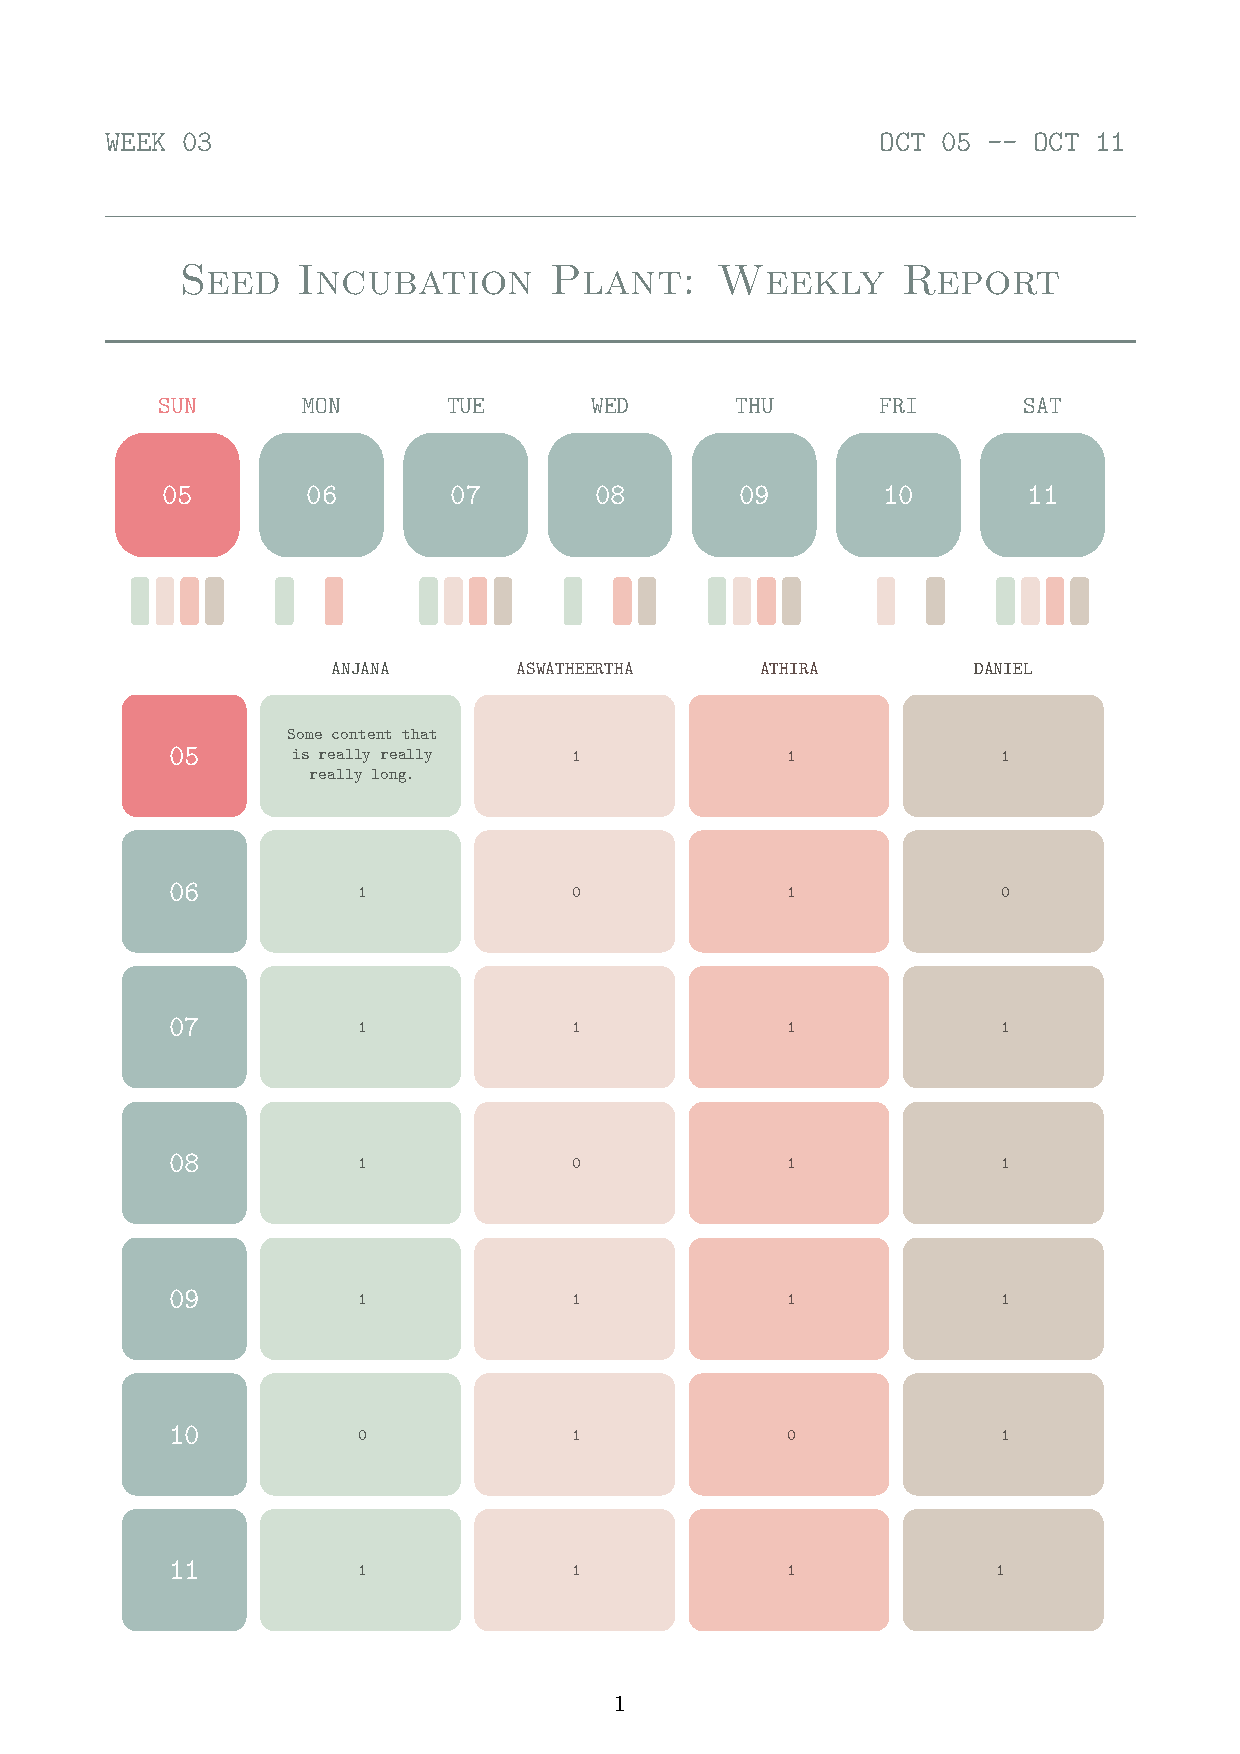
\includegraphics [
            width = 0.30\textwidth,
        ] {wr1.pdf}

        % &
        % 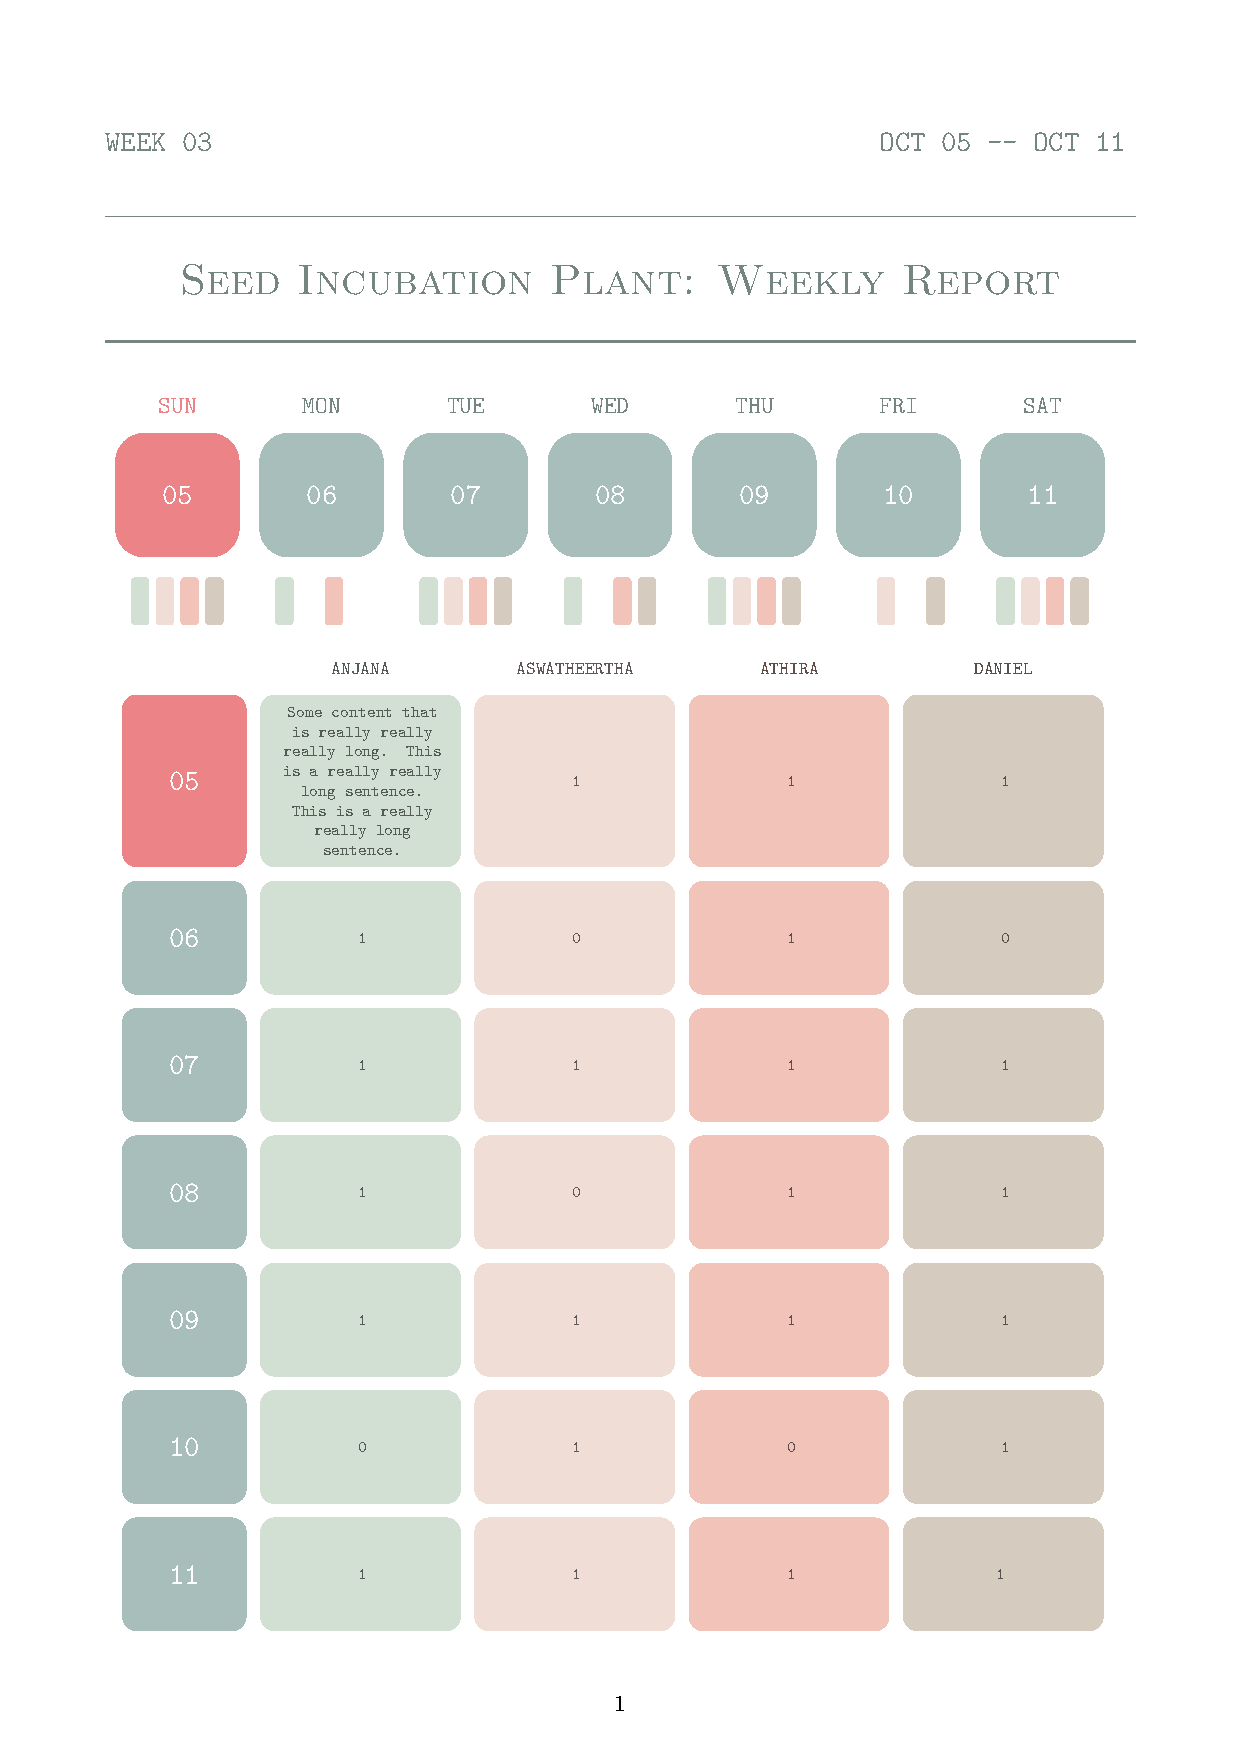
\includegraphics [
        %     width = 0.30\textwidth,
        % ] {wr2.pdf}

        &
        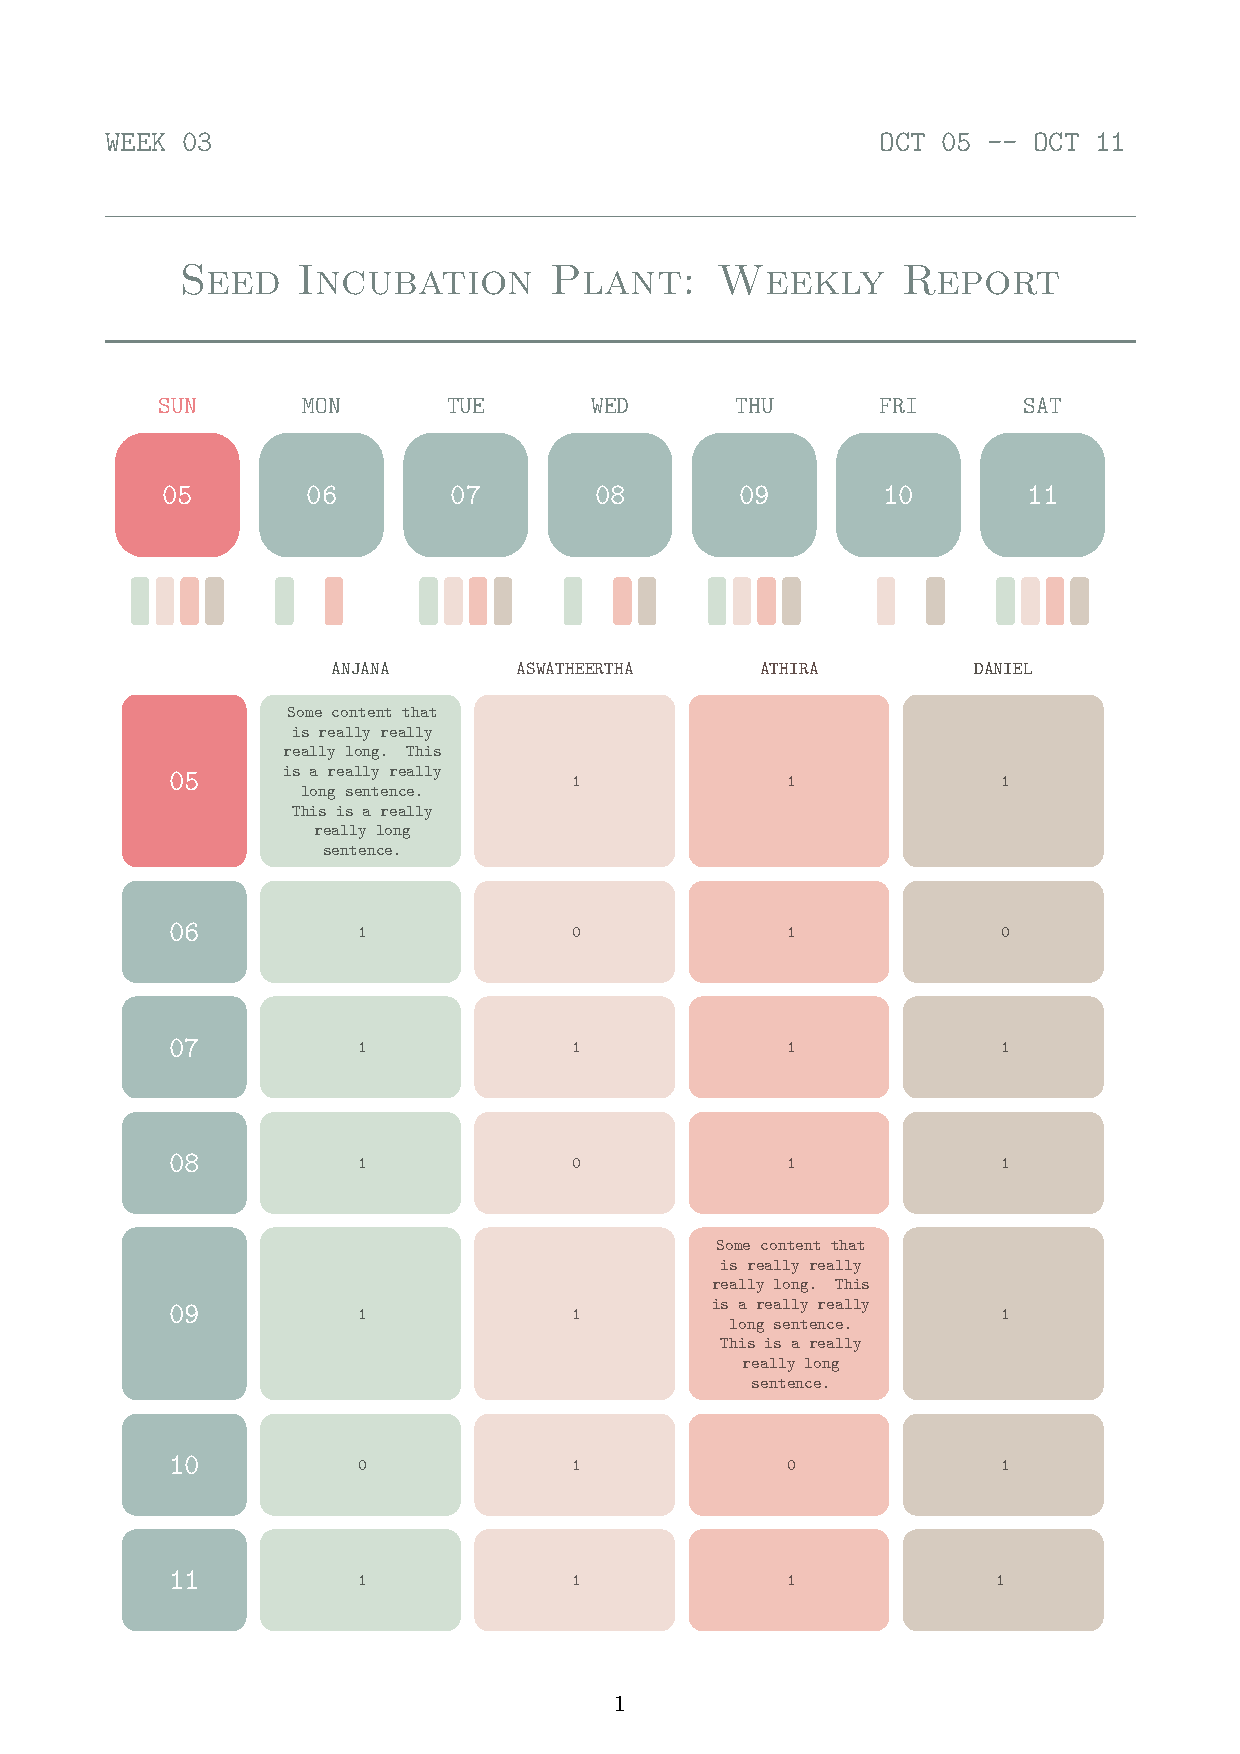
\includegraphics [
            width = 0.30\textwidth,
        ] {wr3.pdf}

        &
        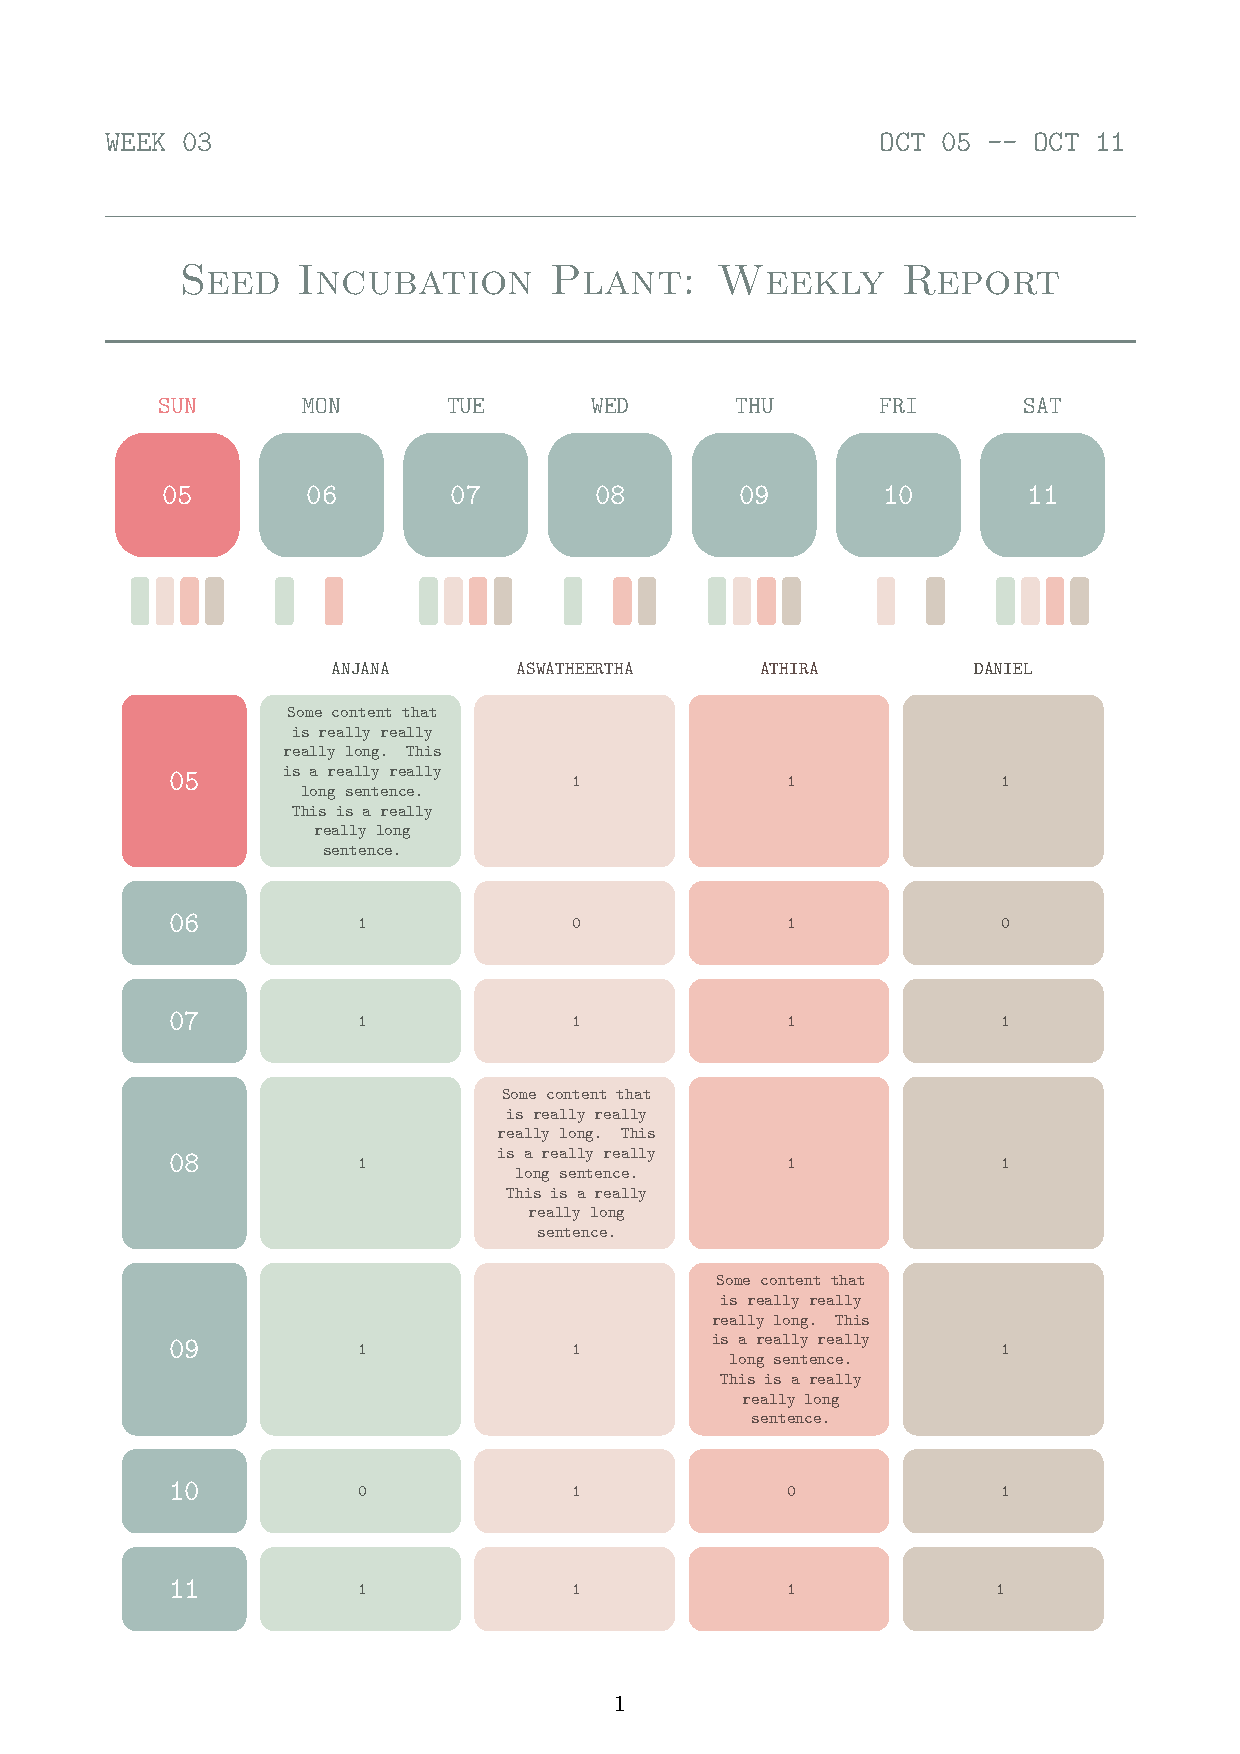
\includegraphics [
            width = 0.30\textwidth,
        ] {wr4.pdf}

        \\

    \end{tabular}
    \captionof{figure} {Auto adjusting overview table.}
    \label{fig:autoAdjustingTable}
\end{center}

\subsection{Figures and Content for Phase One Report}

Most of the figures and content for phase one report is done. This
includes block diagrams, CAD exported figures, annotated figures.
See figure \ref{fig:phaseOneReport} for some of them.

\begin{center}
    \begin{tabular} {
            cc
        }

        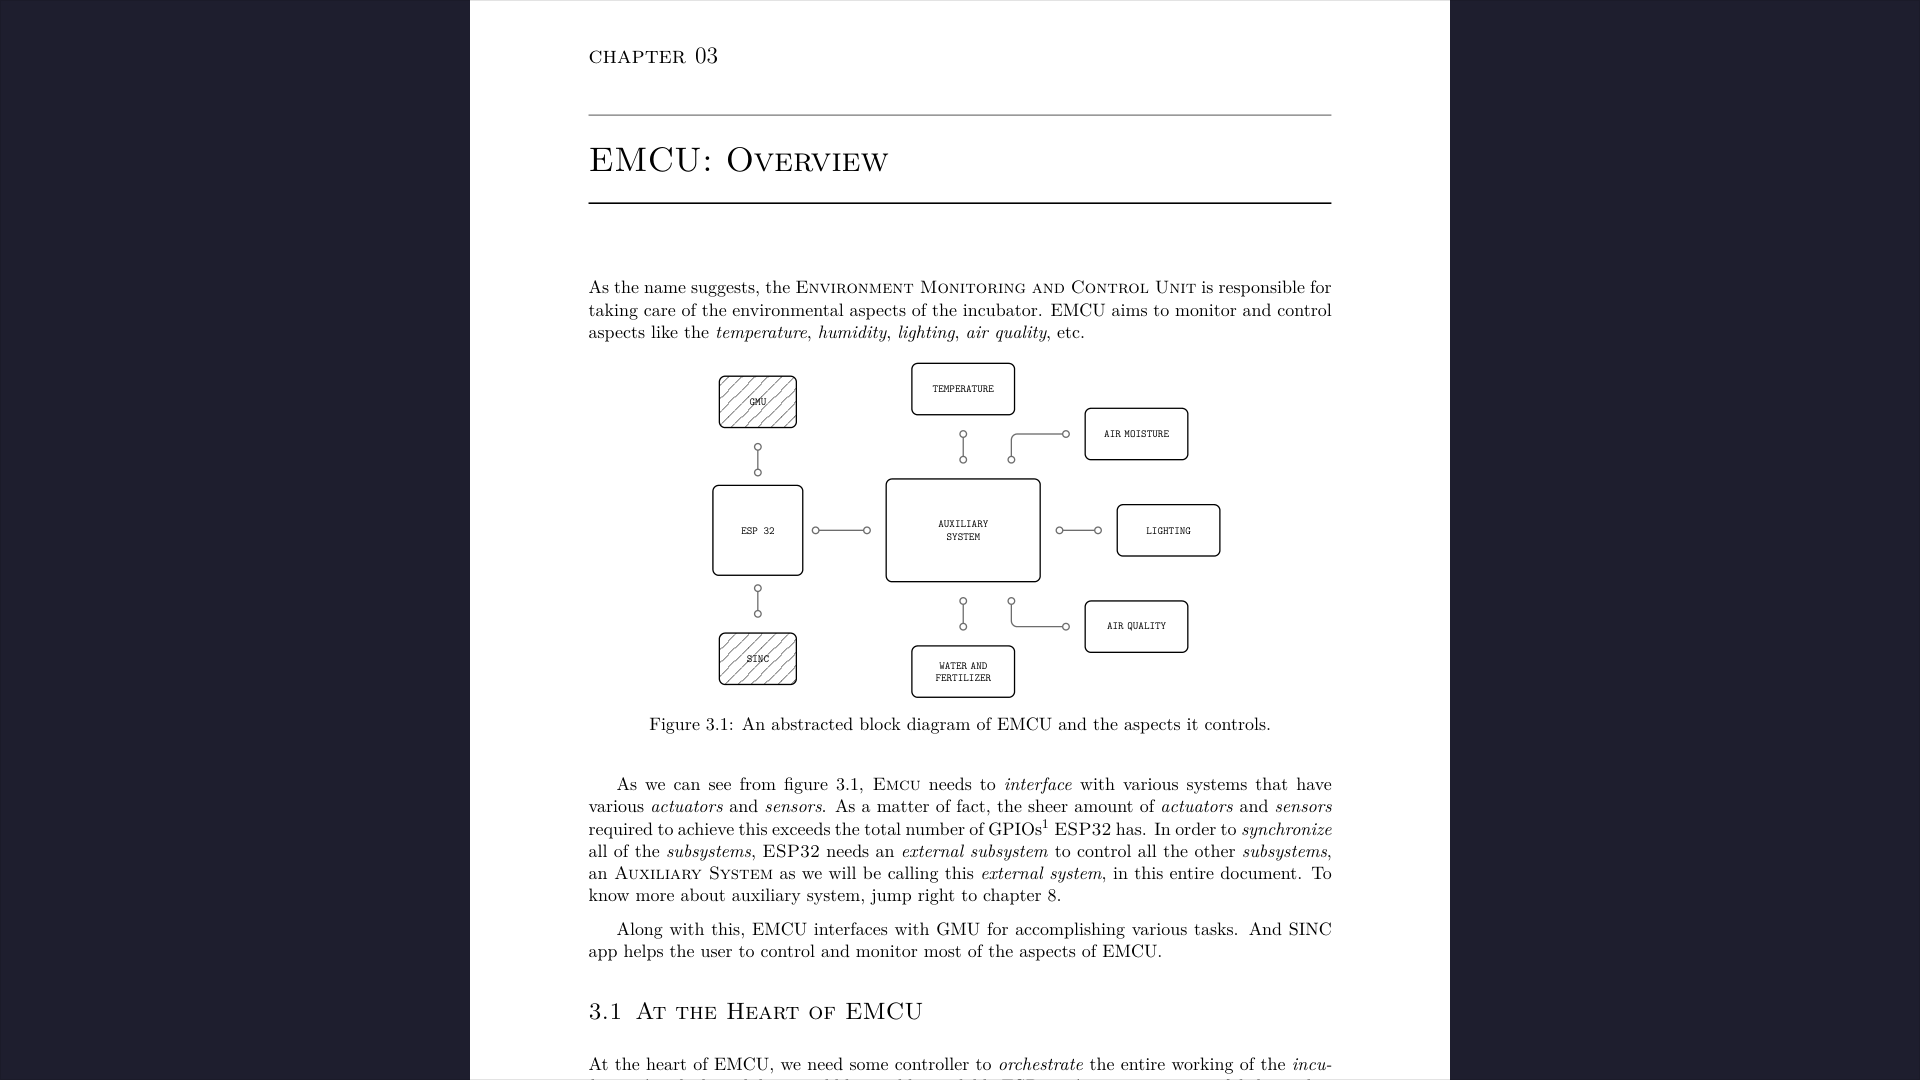
\includegraphics [
            width = 0.45\textwidth,
        ] {ss1.png}

        &
        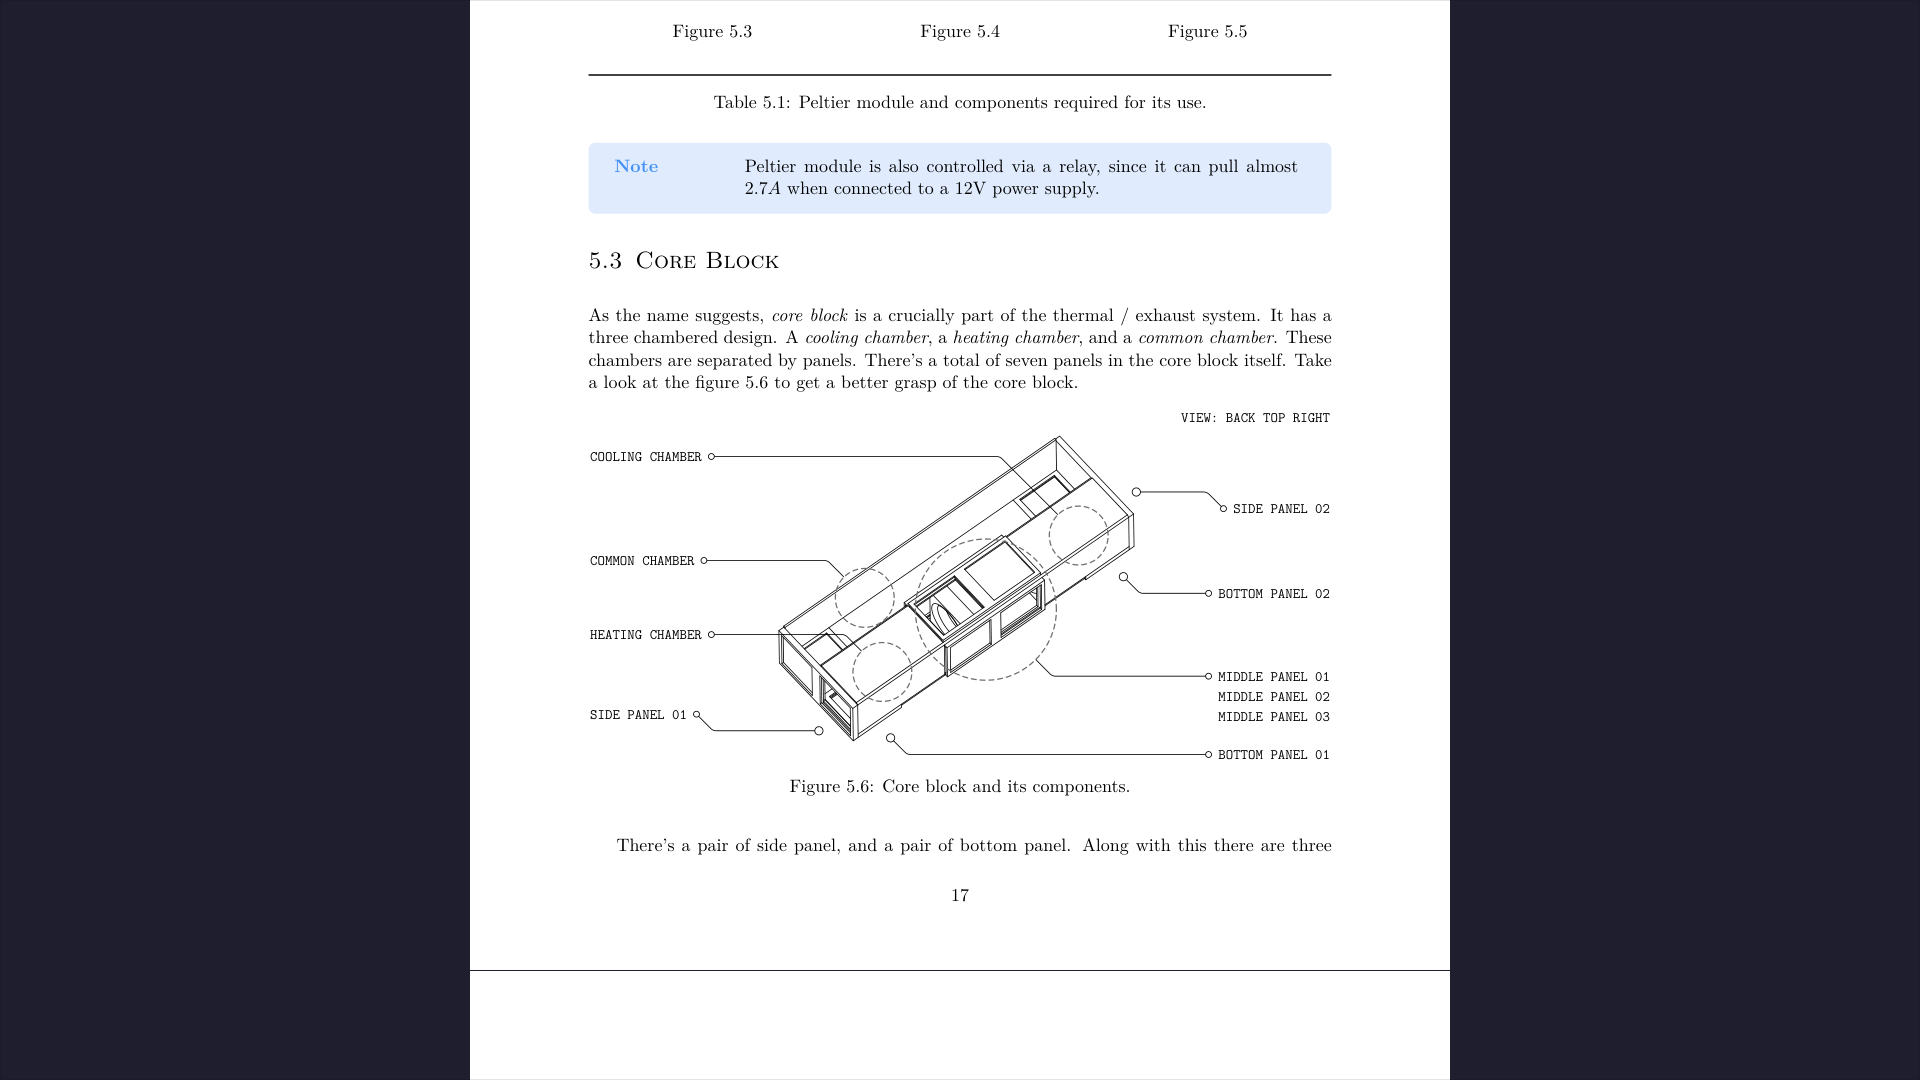
\includegraphics [
            width = 0.45\textwidth,
        ] {ss2.png}

        \\
        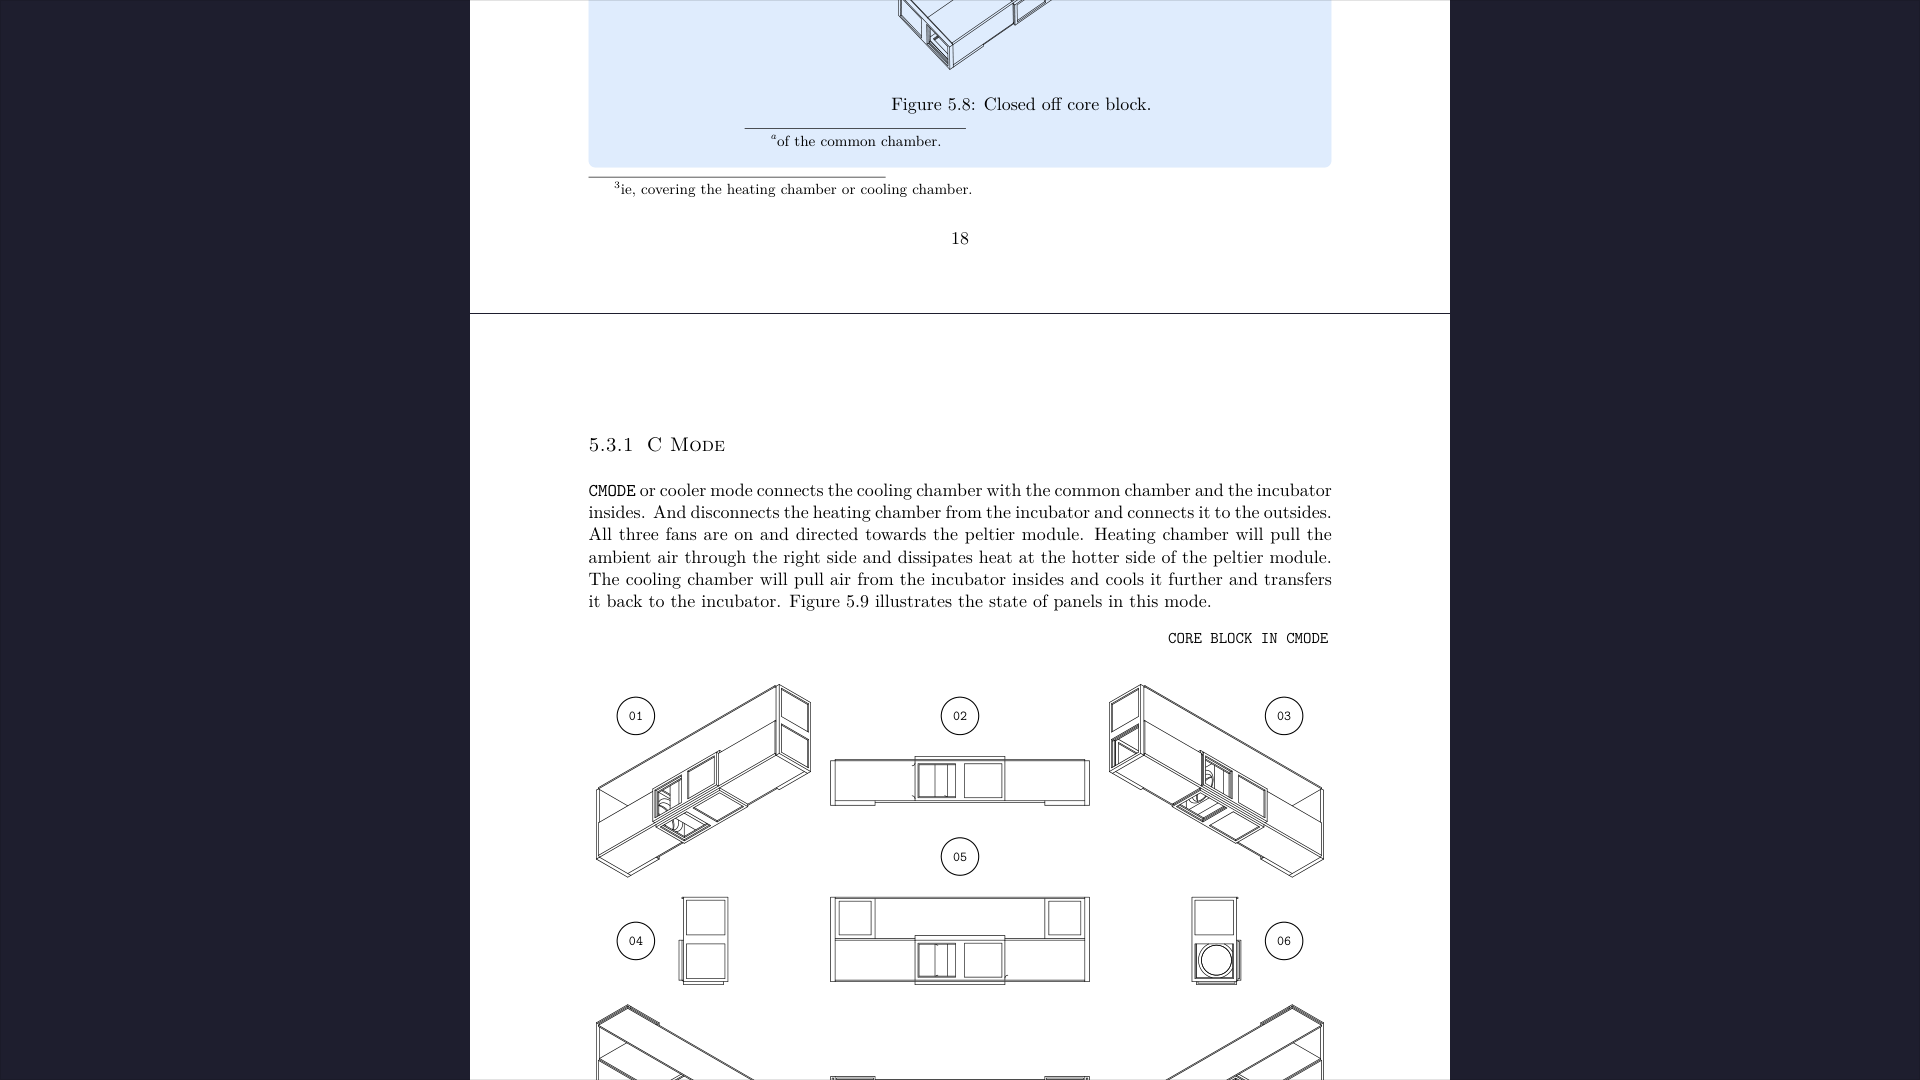
\includegraphics [
            width = 0.45\textwidth,
        ] {ss3.png}

        &
        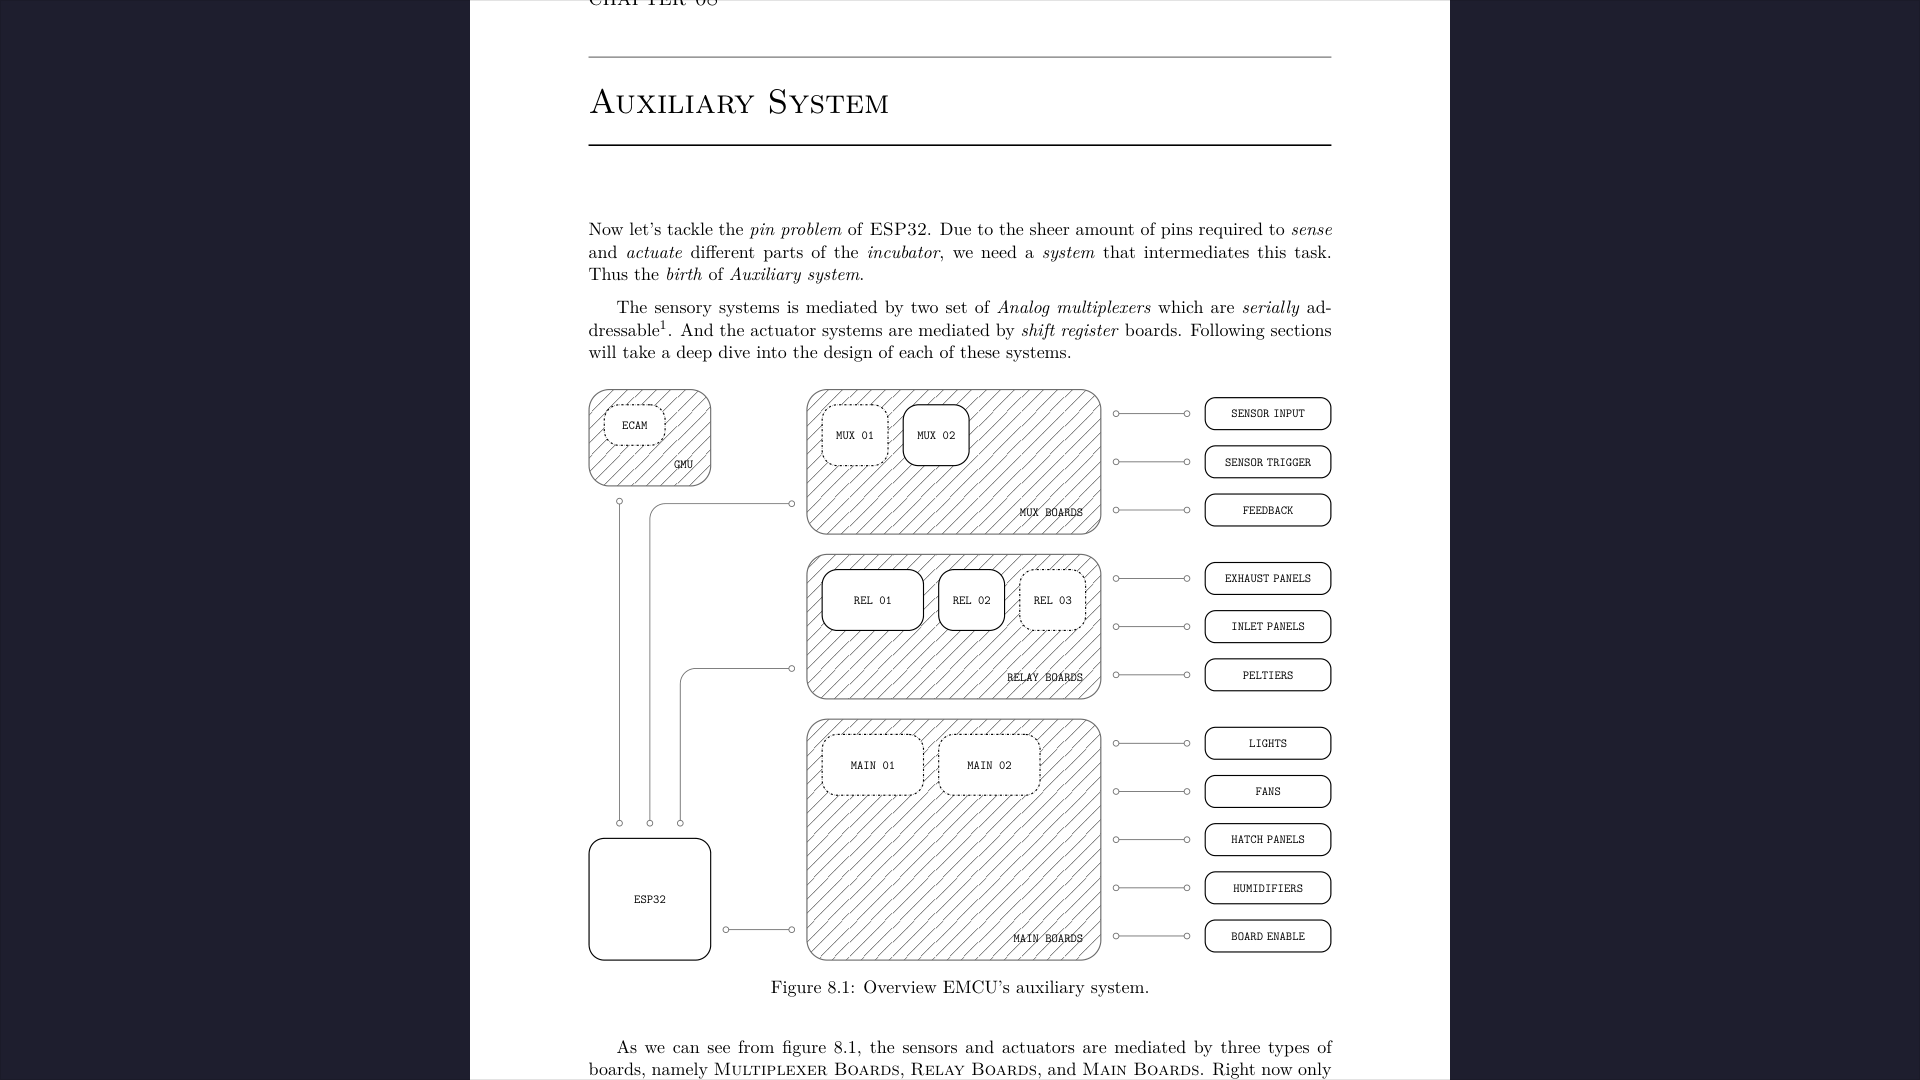
\includegraphics [
            width = 0.45\textwidth,
        ] {ss4.png}

        \\

    \end{tabular}
    \captionof{figure} {Figures and content for project phase one report.}
    \label{fig:phaseOneReport}
\end{center}

\end{document}
